\input{{configplaindocEN.texconf}}

\usepackage{float}

\author{Lucas Haupt\\ Alexander Koschenko\\ David Mertens\\ Dennis Oberst\\ Lena Marie Wilbertz}
\title{Project Schedule PAM3\\ Mobile Hardware Sampler}
\date{\today}

% Style: Sentence Case (only first word in headings capitalized)

\begin{document}
\maketitle

\section{Work packages}

There are three main subprojects that will form the whole project as well as three different project stages in order to roughly structure the overall time available.

\subsection{Subprojects}

\begin{itemize}
\item Midi communication
\item Audio playback and storage
\item Display and user interface
\end{itemize}

\subsection{Stages}

\begin{itemize}
\item Stage 1: Basic function
\item Stage 2: Extended and optional features
\item Stage 3: Casing and final product
\end{itemize}

\subsection{Detailed description}

\begin{itemize}
	\item Audio playback and storage

		Making the audio playback and storage of samples work.
		This will involve some parallel programming as well as
		getting the flash chip to work (soldering and setting up).

	\item Sample selection with rotary encoder

		Connecting the rotary encoder to the Teensy and programming it
		to select a certain sample from the flash storage. Selection of
		a sample will be dependent on the preceding work package, selection
		in general could be tested by using a dummy programm (ui only).

	\item Displaying selected sample names

		This is partly dependent on the preceding sample selection but mainly
		aimed at getting the display to work and rendering text on it.

	\item Menu design (structure and visuals)

		Dependent on the preceding work package. Menu design and user interface design
		are closely connected to the arrangement of buttons and the type of display 
		in use. The main aspect of this work package will be finding a creative and
		usable solution to make the interaction with the final product work intuitively
		and easy.

	\item Line out playback

		This is dependent on the audio playback. Main challenge will be soldering
		proper connectors and testing the audio line.

	\item Recording with line in and mic

		This is also dependent on the playback work package. Here, soldering is also
		a main task as well as some programming challenges with the goal to add
		recording abilities over line in and mic.

	\item Master volume control

		Dependent on line out playback package. This package aims to provide a
		volume control for the headphone and line out. Task will be to extend menu
		and program to provide a button/menu function to lower and raise output volume.

	\item Midi connection over DIN 5 connector

		This work package deals with the Midi part of the project. Here, Midi connectors
		should be attached to the Teensy and it should be possible to trigger midi notes
		with an external midi device over the DIN 5 connector.

	\item Digital effects and filters (at least 2)

		This work package deals with adding digital effects and filters in order to
		change the sound of the samples being played.

	\item Menu extension: controlling effects

		This work packages is dependent on the digital effects wp and deals with extending
		the menu to provide an interface for controlling effect parameters.

	\item Adding 4 velocity sensitive pads

		This work package aims to add velocity sensitive pads in order to trigger samples with
		the help of these pads and make the sampler a mobile standalone device.

	\item Recording midi

		Recording midi snippets is the goal of this work package.

	\item 2-8 voice polyphony

		Adding the possibility of playing multiple samples/notes at once.
		
	\item Case design and crafting

		Creating an eyecatching and usable case and finding parts and materials to craft it.

	\item Pcb assembly

		Designing the Pcb and assembling the parts in a way that fits the case.

	\item Device assembly (case + pcb)

		This work package aims to put pcb and case together and thus is dependent on the last two wps.
\end{itemize}



\section{Milestone/Task list}

\begin{figure}[H]
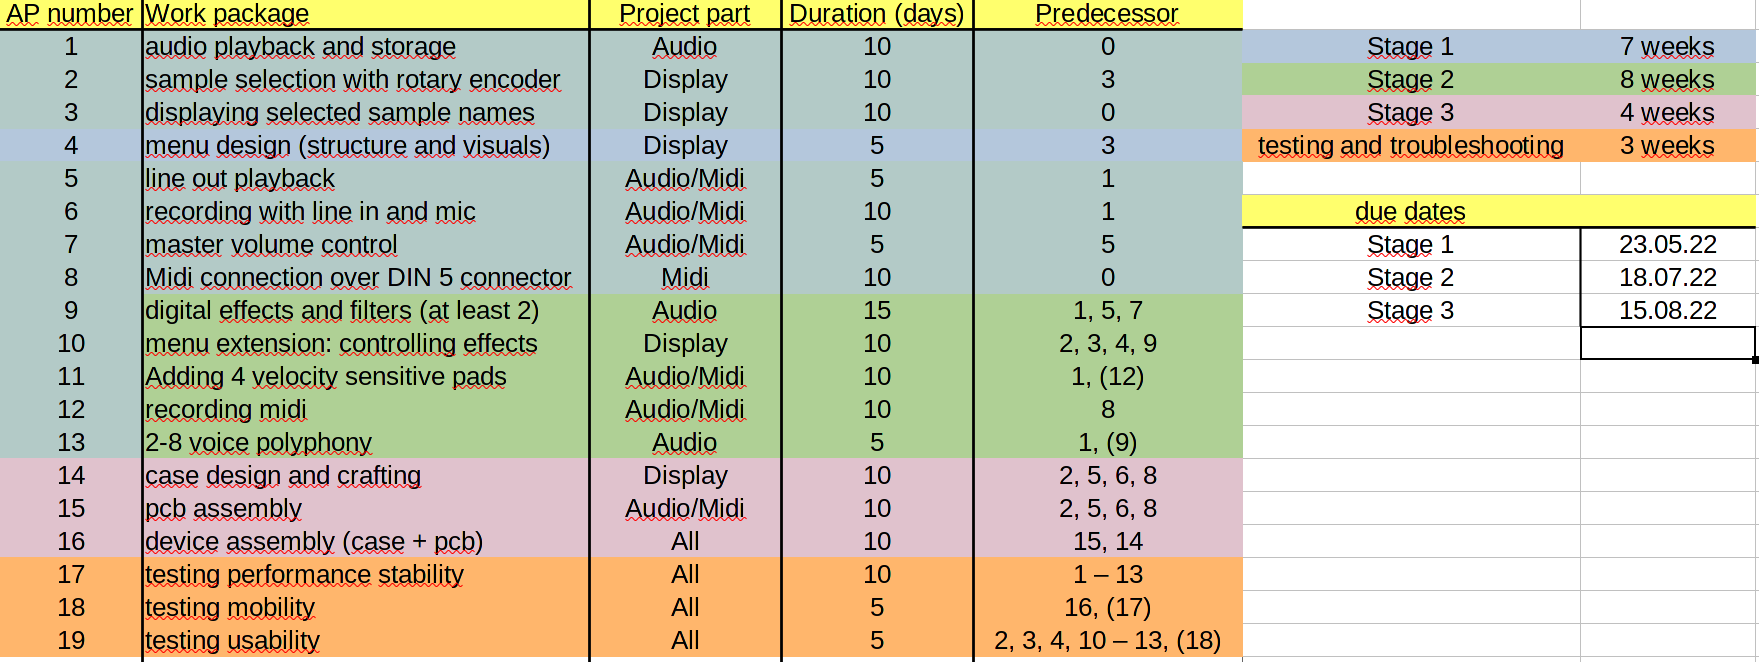
\includegraphics[width=\textwidth]{task_list.png}
\caption{Task list}\label{fig:task}
\end{figure}

\section{Gantt chart}

\begin{figure}[H]
\centering
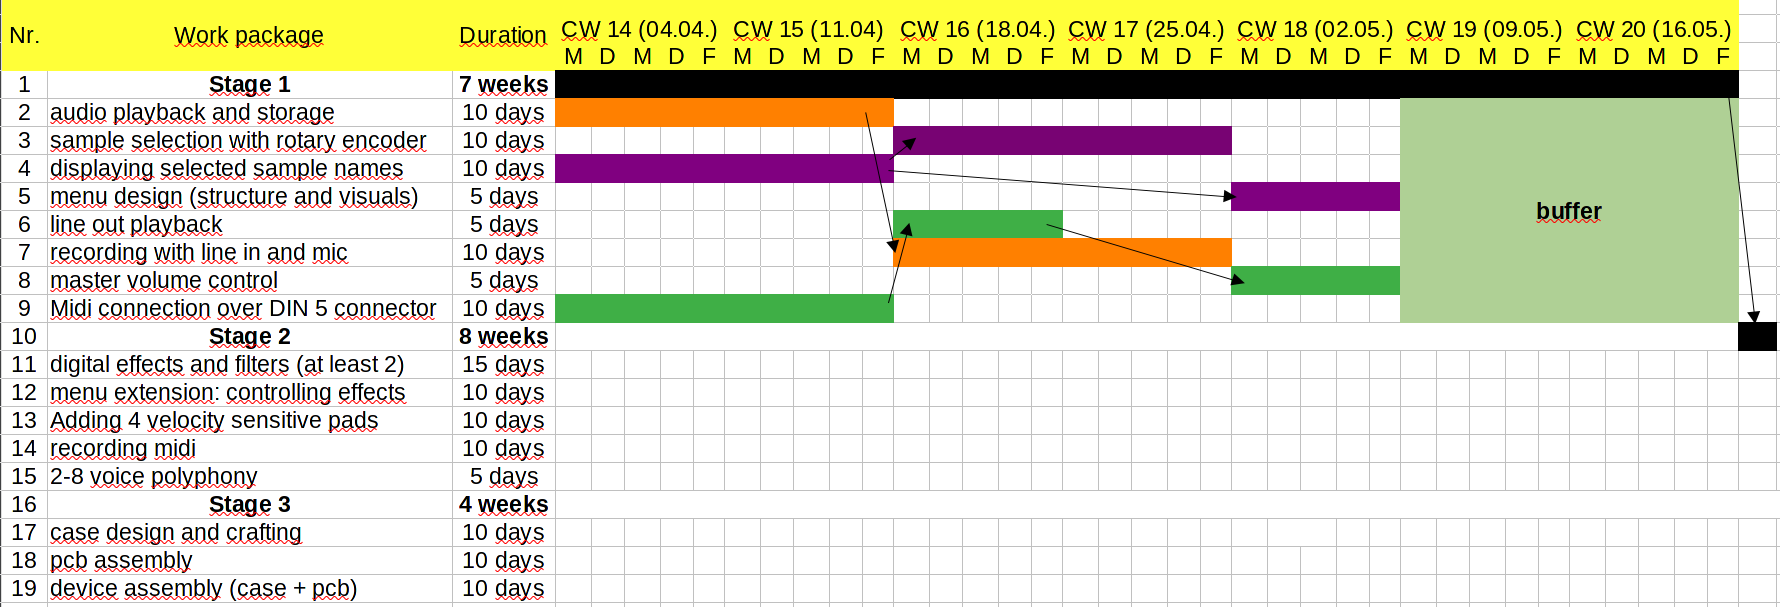
\includegraphics[width=\textwidth]{gant_chart01.png}
\\
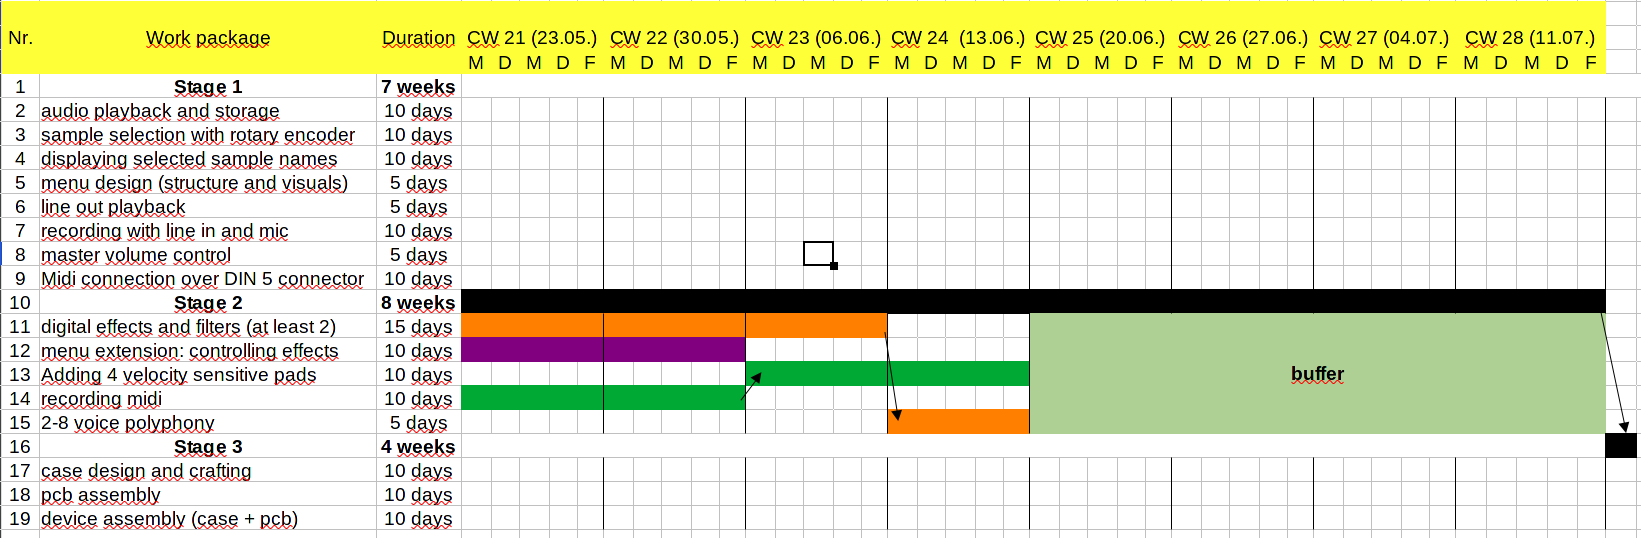
\includegraphics[width=\textwidth]{gant_chart02.png}
\\
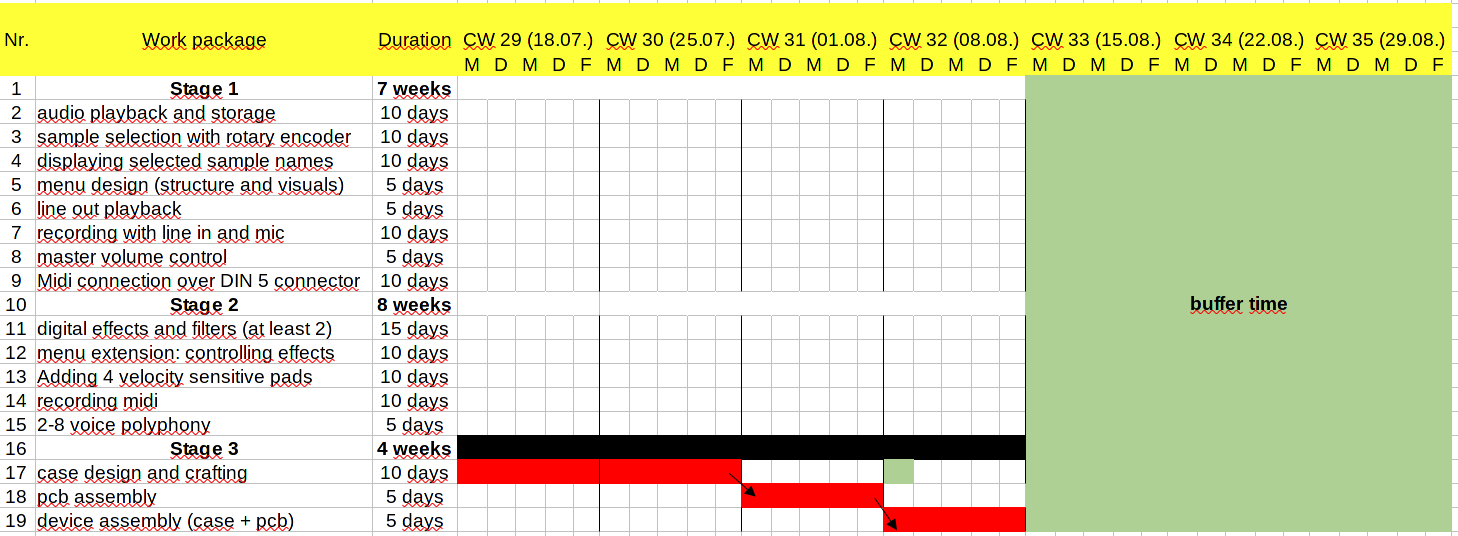
\includegraphics[width=\textwidth]{gant_chart03.png}
\caption{Gantt chart}\label{fig:gntt}
\end{figure}

\section{Precedence diagram}

\subsection{Stage 1}
\begin{figure}[H]
\centering
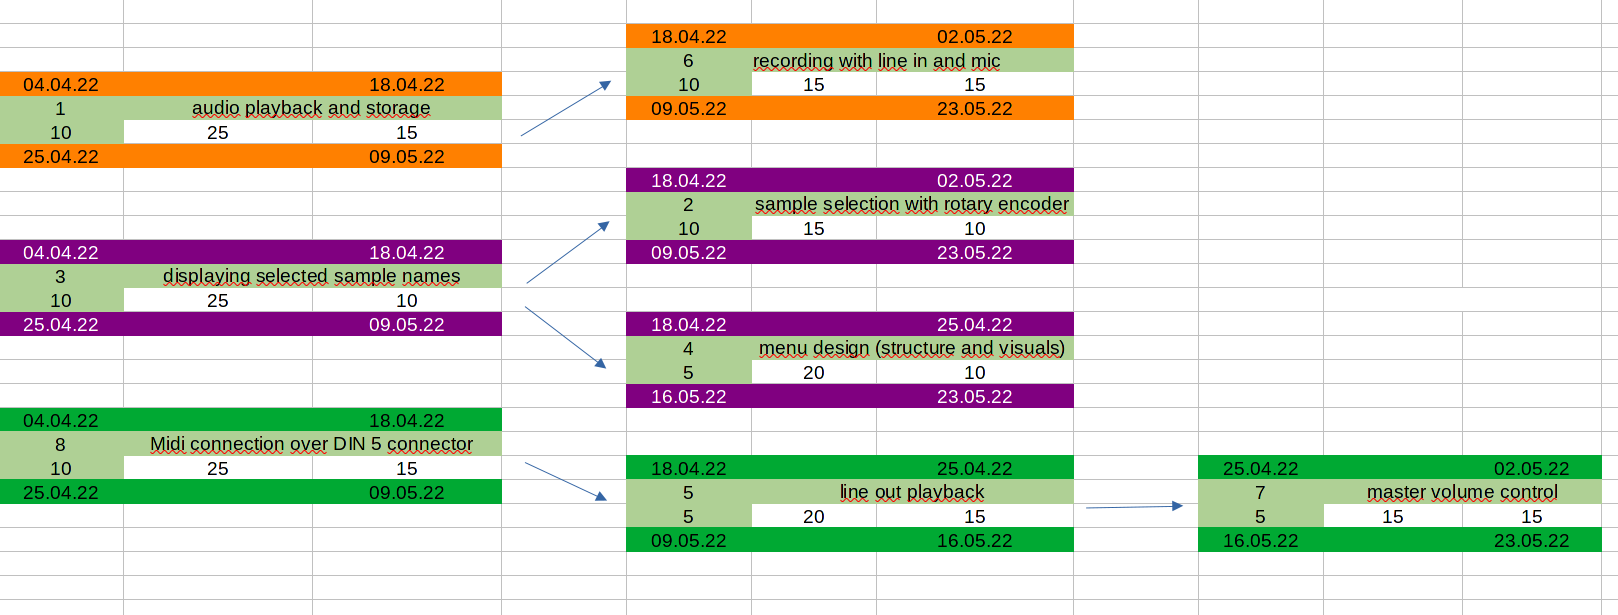
\includegraphics[width=\textwidth]{prec_chart01.png}
\caption{Precedence diagram stage 1}\label{fig:prec01}
\end{figure}

\subsection{Stage 2}
\begin{figure}[H]
\centering
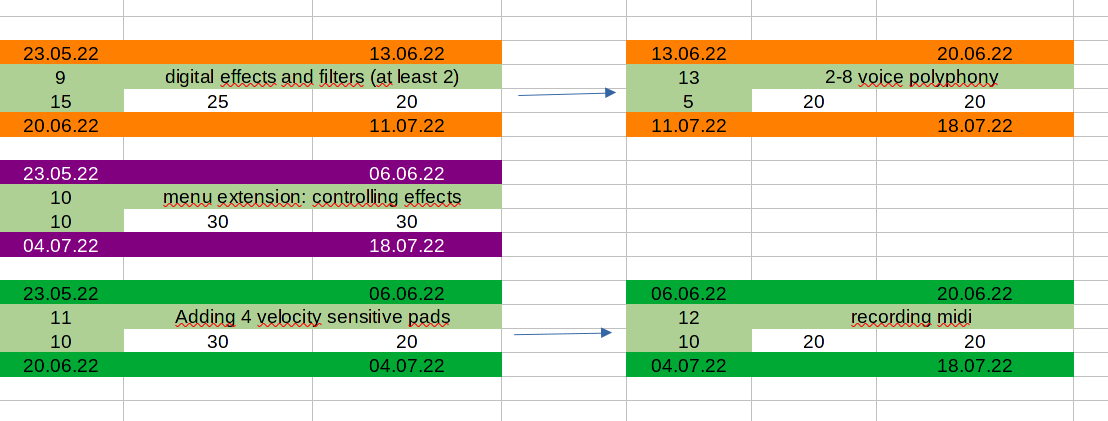
\includegraphics[width=\textwidth]{prec_chart02.png}
\caption{Precedence diagram stage 2}\label{fig:prec02}
\end{figure}

\subsection{Stage 3}
\begin{figure}[H]
\centering
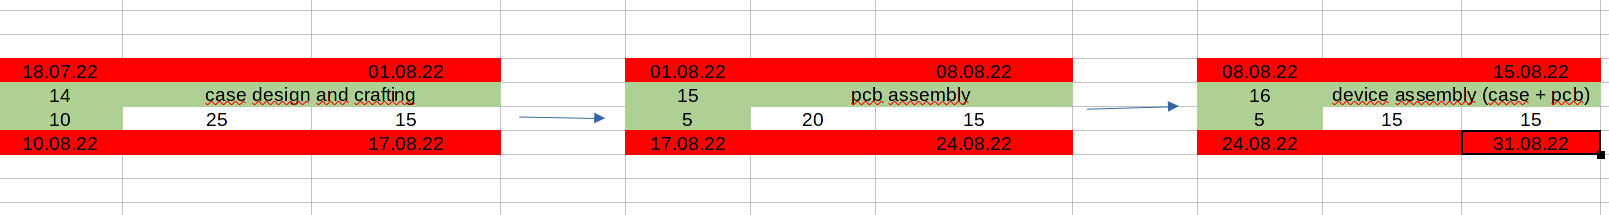
\includegraphics[width=\textwidth]{prec_chart03.png}
\caption{Precedence diagram stage 3}\label{fig:prec03}
\end{figure}

\end{document}
